\setlength{\headheight}{15pt}
\addtolength{\topmargin}{-2.5pt}

\chapter{Technology Review}

\section{Executive Dashboard}
When it came to developing the Executive Dashboard for data analysis it was crucial to select the tools that could transform data into easily comprehensible information. After conducting research and exploring alternatives Angular and Chart.js were chosen for specific reasons.

\subsection{Angular}
Angular is based on TypeScript and is an open-source framework, and it's a great tool for building client-side web applications. It can be used for single-page applications (SPAs) or for enterprise-level solutions. 

\subsubsection{Main Concepts: Components, Modules and Services}
Angular is composed of three foundational blocks: Components, Modules and services.

\subsubsection{Components} Components are like Lego blocks of the application. Each component holds a portion of the user interface and its behaviour. Components serve as the bridge between the application data and what the user experiences on the screen.\cite{angular-components}

\subsubsection{Modules} In Angular modules serve as containers that group related components, directives, and services together that can be combined with other modules. It plays an important role in improving maintainability and re-usability, key concepts of Angular development.\cite{angular-modules}

\subsubsection{Services} Angular services use typescript classes with injectable decorators. The decorator tells angular that the class is a service and can be injected into other components that need that service.\cite{angular-services}


\subsection{Angular architecture}
Angular uses the Model-View-Controller (MVC) pattern, with a variation known as Model-View-ViewModel (MVVM). The controller is responsible for the interaction between the model and the view.

\begin{figure}[ht]
    \centering
    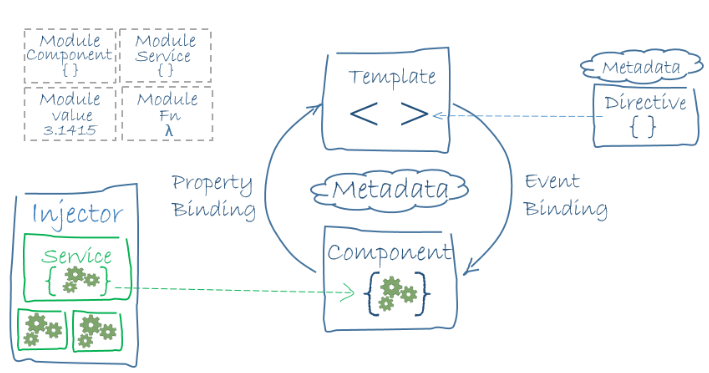
\includegraphics[width=0.85\linewidth]{images/angular-arch.png} 
    \caption{Angular application architecture}
    \label{fig:angular-arch}
\end{figure}

\subsection{Advantages of using Angular}
\subsubsection{Component-Based Architecture} 
 As mentioned earlier in discussions Angular organisess its functionalities into components. These components have the ability to communicate with each other enabling updates to sections without affecting the rest of the application.

\subsubsection{Mobile-Friendly Approach} 
Angular incorporates techniques such, as lazy-loading, which means loading parts of the application (like images) only when they are needed. This ensures that users do not experience long waiting times.

\subsubsection{Two-Way Data Binding} 
With Angular two way data binding data can seamlessly flow between the component and the view allowing for synchronization.

\subsubsection{Asynchronous Programming} 
By utilizing programming executes code in a non-sequential manner and employs multi-threading to enhance performance. This speeds up operations and prevents system freezes, providing users with a seamless experience.
 
\subsubsection{Single-Page Applications}
Angular creates a dynamic single-page application which can be navigated without page reloads, improving the user experience with better user interaction and engagement.

\subsubsection {Code Re-usability} 
The component-based architecture of Angular promotes the re-usability of UI components saving development time.

\subsubsection{Dependency Injection} 
With dependency injection in place, Angular allows for the creation of objects that rely on other objects. This improves modularity and efficiency, within the app.

\subsubsection{Angular Material} 
Angular's documentation offers a range of built user interface components and modules that adhere to Google's Material Design principles. This greatly facilitates the developer's work, simplifying the design process and enabling application development.

\subsubsection{Angular CLI} Angular command line interface gives the developer the ability to generate Angular projects, modules, services, and components with a single command, this not only saves time but also reduces configuration errors, it gives the developer the freedom to dive into creative aspects of the project, focusing on innovation and functionality rather than getting bogged down by initial setup complexities.

Angular command line interface gives the developer the ability to generate Angular projects, modules, services, and components with a single command, this not only saves time but also reduces configuration errors, it gives the developer the freedom to dive into creative aspects of the project, focusing on innovation and functionality rather than getting bogged down by initial setup complexities.

\section{Data Visualization}

Data visualization is the process of translating large volumes of data into visual representations. It is a powerful tool that allows for the identification of patterns and trends that would otherwise be difficult to identify. It is a key component of data analysis and is used to communicate information clearly and efficiently.

\subsection{Chart.js}
Chart.js is robust, lightweight and open source javascript library that provides features for creating visually appealing charts and graphs that can be embedded into a web page. It is a great tool for data visualization and is easy to use. It is based on HTML5 canvas and is responsive, meaning that the charts will adapt to the size of the container element. It is also compatible with all modern browsers and is supported by a large community of developers. \cite{da2019learn}
It can be compared like a the artist's toolkit for developers, providing a flexible API to create a variety of chart types, such as line charts, radar charts, pie charts and many more. It also provides a range of customization options, allowing developers to create unique and visually appealing charts. \cite{da2019learn}

Table \ref{tab:chart-js-features} is showing some of the features of Chart.js\cite{da2019learn}:

\begin{table}[H]
    \centering
    
    \begin{tabularx}{\textwidth}{|l|X|}
        \hline
        \textbf{Feature} & \textbf{Description} \\
        \hline
        Easy to use & Aesthetically charts can be created without the need of extensive configuration. The library follows a declarative approach allowing the developer to define the data and settings of the chart in a single object. \\
        \hline
        Responsive & Charts generated by Chart.js are responsive, adapting to different screen sizes and devices, ensuring that the visualization remains accessible and readable across various platforms. \\
        \hline
        Customization & Chart.js provides a high degree of customization. Colors, fonts, and other visual elements can be customized to create unique and visually appealing charts. \\
        \hline
        Interactivity & Chart.js provides built-in support for tooltips and animation, allowing the user to explore data points, adding a layer of engagement to the project. \\
        \hline
        Cross-browser compatibility & Chart.js is compatible with all modern browsers, including Chrome, Firefox, Safari, Edge, and Internet Explorer 11. \\
        \hline
    \end{tabularx}
    \label{tab:chart-js-features}
    \caption{Chart.js Features}
\end{table}


Chart.js is a reliable and effective tool for data visualization, it is also easy to use and provides a range of customization options. It is also supported by a large community of developers, which is a great advantage.

\subsection{D3.js}
D3.js or Data-Driven Documents is a JavaScript library for manipulating documents based on data. It has the ability ti bind data to the DOM (Document Obect Model) and creates interactive and dynamic visualization. It provides a lower level and more granular approach to data visualization, giving the developer more control over the visualization process.\cite{d3}


Table \ref{tab:d3-js-features} is showing some of the features of D3.js\cite{d3}:

\begin{table}[H]
    \centering
    
    \begin{tabularx}{\textwidth}{|l|X|}
        \hline
        \textbf{Feature} & \textbf{Description} \\
        \hline
        Data-Driven & D3.js is data-driven, meaning that it can bind data directly to HTML or SVG elements. This type of control is advantageous for creating highly customized visualizations. \\
        \hline
        Modular & D3.js is modular, composed of many small modules that can be used independently or combined together to create a custom visualization. \\
        \hline
        Extensible & D3.js is extensible, meaning that it can be extended to support any type of visualization. \\
        \hline
        Community & D3.js is supported by a large community of developers, which is a great advantage. \\
        \hline
    \end{tabularx}
    \label{tab:d3-js-features}
    \caption{D3.js Features}
\end{table}


D3.js is a powerful tool for data visualization, it provides a high degree of customization and control over the visualization process. However, it is more complex and requires more time to learn and implement. It is also not supported by all browsers, which is a disadvantage.

In conclusion, while D3.js is a powerful tool for data visualization, it is more complex and requires more time to learn and implement. It is also not supported by all browsers, which is a disadvantage. Considering the scope of the project and the time constraints, Chart.js was chosen as the tool for data visualization. It is easy to use and provides a high degree of customization, allowing for the creation of unique and visually appealing charts. It is also supported by a large community of developers, which is a great advantage.

\section{AI module - Data analysis}
Ninety per cent of the world's data was generated in just the last two years. In the early 2000s, the amount of data being generated exploded exponentially with the use of the internet, social media, and various other technologies. Organizations found themselves facing a massive volume of data that was very hard to process. To address the challenge, the concept of Big data emerged. Big data refers to extremely large and complex data sets that are difficult to process using traditional methods. \cite{bigdata}

\subsection{Hadoop}
As the volume of data grew rapidly across the globe, organizations needed a way to manage it to gain valuable insights. That’s where Hadoop came in. In 2006, a team of engineers from Yahoo developed Hadoop inspired by Google’s MapReduce. Hadoop has introduced a new way of handling data called distributed processing. Now, to process all data it wouldn't use single machines anymore, instead, Hadoop uses multiple computers, allowing large amounts of data to be processed way faster than before.
Hadoop has mainly two main components: HDFS (Hadoop Distributed File System) and MapReduce. HDFS stores the into multiple computers, and MapReduce is responsible for processing the data in parallel allowing the organizations to store and process large amounts of data.
Hadoop was a great advance in big data processing, however, it had a few limitations. One of the biggest problems was that it relied on storing data on disk. This slowed down data processing because every time a job ran it had to save its data to disk, read it back, process it, and save it back to disk Another problem is that Hadoop processes data only in batches. This means a new job couldn't be submitted before the other job ended.
With Hadoop, storing and processing large amounts of data became possible, even with some limitations it was an important step in big data processing.\cite{hadoop}


\subsection{Apache Spark}
As described Hadoop has a few limitations, there was a need to process all this data faster and in real-time. And here is where Apache Spark comes into action. In 2009, researchers at the University of California developed Apache Spark as a research project. At this point, RDD (Resilient Distributed Dataset) was introduced and deemed to be a very powerful concept.\cite{apache-spark}
RDD is the backbone of Apache Spark, storing the data in memory for faster access and processing. It will not read and write the data from the disk, instead, Spark processes the entire data just in memory. The meaning of memory here is the RAM (Random Access Memory) stored inside the computer. This in-memory data processing of data makes Spark much faster than Hadoop. 
Spark also gives the ability to write code in various programming languages such as JAVA, Scala, Python and R, along with an optimized engine that supports general execution graphs.

\subsubsection{Main components and Features}

\begin{figure}[ht]
    \centering
    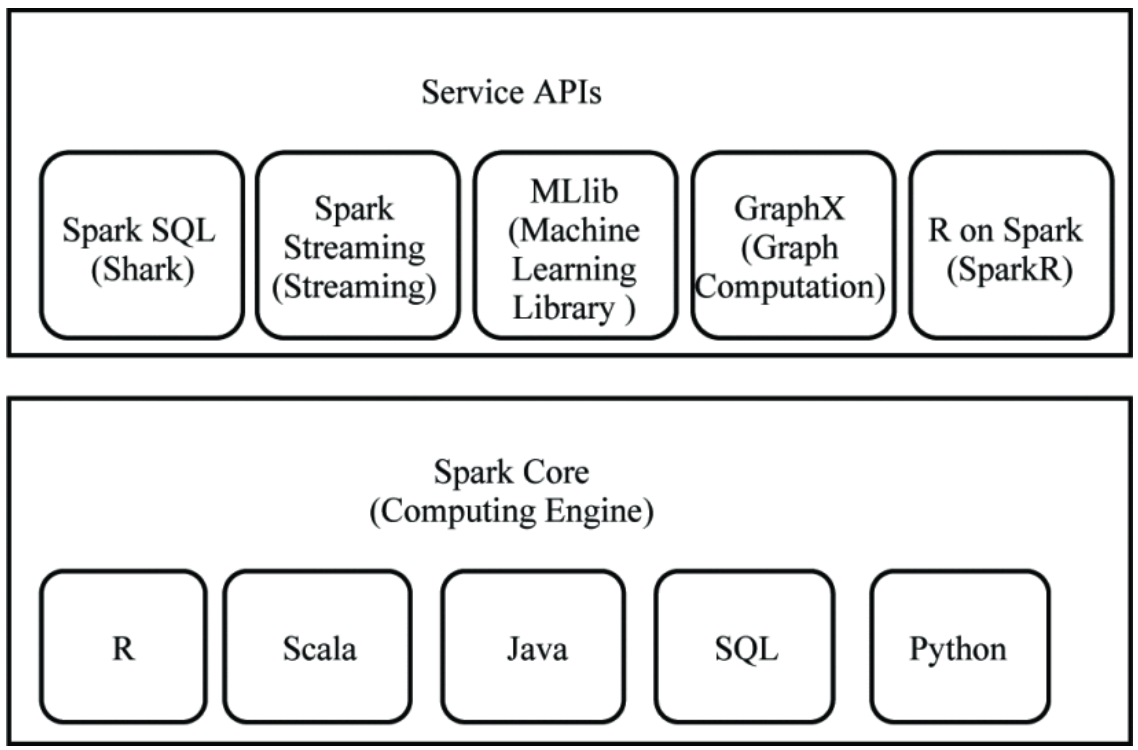
\includegraphics[width=1\linewidth]{images/Spark_Eco.png}
    \caption{Apache Spark Ecosystem}
    \label{fig:spark-eco}
\end{figure}

The Apache Spark ecosystem consists of the following main components\cite{8988541}:
\begin{itemize}
    \item Spark SQL: Formerly known as Shark.  Spark SQL is a distributed framework that works with structured and semi-structured data. It facilitates analytical and interactive applications for both streaming and historical data which can be accessed from various sources such as JSON, Parquet and Hive table.\cite{8988541}
    \item Spark Streaming: Allows to process real-time data. Is a scalable fault-tolerant streaming processing system that supports both batch and streaming workloads. Spark streaming enhances the fast scheduling capability of Apache Spark by inserting data into mini-batches. An operation known as transformation is then applied to those mini-batches that can be easily obtained from live streams and data sources such as Twitter, Apache Kafka, IoT sensors, and Amazon Kinesis.\cite{8988541}
    \item Spark Core: One of the most important parts of the Spark ecosystem is called Spark Core. It helps process data across multiple computers and ensures everything works efficiently and smoothly. Various functionalities of Apache Spark are built on top of the Spark core. It provides a vast range of APIs as well as applications for programming languages such as Scala, Java, and Python APIs to facilitate the ease of development. In-memory computation is implemented in Spark core in order to deliver speed and solve the issue of MapReduce.   
    
    \item MLlib: It delivers high-quality algorithms with high speed and makes machine learning easy to use and scale. Several machine learning algorithms such as regression, classification, clustering, and linear algebra are present. It also provides a library for lower-level machine learning primitives like the generic gradient descent optimization algorithm. It also provides other functions such as model evaluation and data import. It can be used in Java, Scala, and Python. \cite{8988541}
\end{itemize}

With all these components working together, Apache Spark became a powerful tool for processing and analysing Big Data. Spark manages and coordinates the execution of tasks on data across a cluster of computers. 

\begin{figure}[ht]
    \centering
    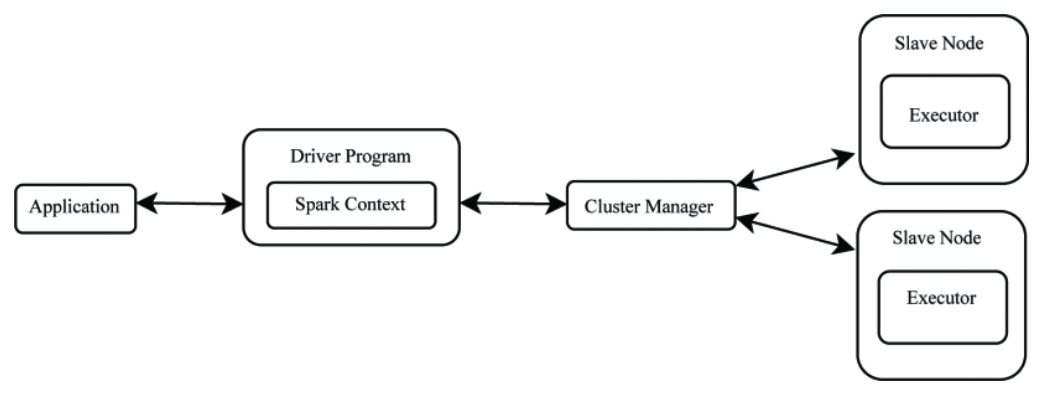
\includegraphics[width=1\linewidth]{images/Spark_Arch.png} 
    \caption{Apache Spark Architecture}
    \label{fig:spark-arch}
\end{figure}

Figure~\ref{fig:spark-arch} shows the Spark Architecture. It consists of a master node which has a driver program that is responsible for calling the main program of an application, this driver could be the Spark shell or the application, written in Scala or Java, for example. It is basically the entry point and is responsible for creating Spark context, which behaves like a gateway to all of the functionalities of Apache Spark. It allows for communication and coordination with other nodes within the cluster, known as Slave nodes. Within the slave node, there are many numbers of executors which act as workers. Whenever a job is initiated, the driver process will make sure it goes through the Apache application properly. It analyzes the work that needs to be done, divides it into smaller tasks and assigns it to the executors. The driver process is the heart of the Apache Spark application and executors are the real workers, which execute the work assigned by the driver and report back the progress and results of the computation.\cite{8988541}

Due to the powerful capabilities of distributed computing, large volumes of data can be processed quickly and efficiently. For all these reasons, it was deemed to be the perfect technology to be used in this project. As the project evolves and more data is gathered from our research volunteers, Spark's performance scales with the size of the data, processing with high speed.


\subsection{Node JS}

\subsection{Docker}

\subsection{PM2}

\subsection{NGINX}

\subsection{MySQL}

\subsection{Express JS}

\subsection{TensorFlow}

\subsection{AWS Services}

